\subsection{M.PD.12 - Adeguatezza delle funzioni sviluppate}

\begin{figure}[H]
  \centering
  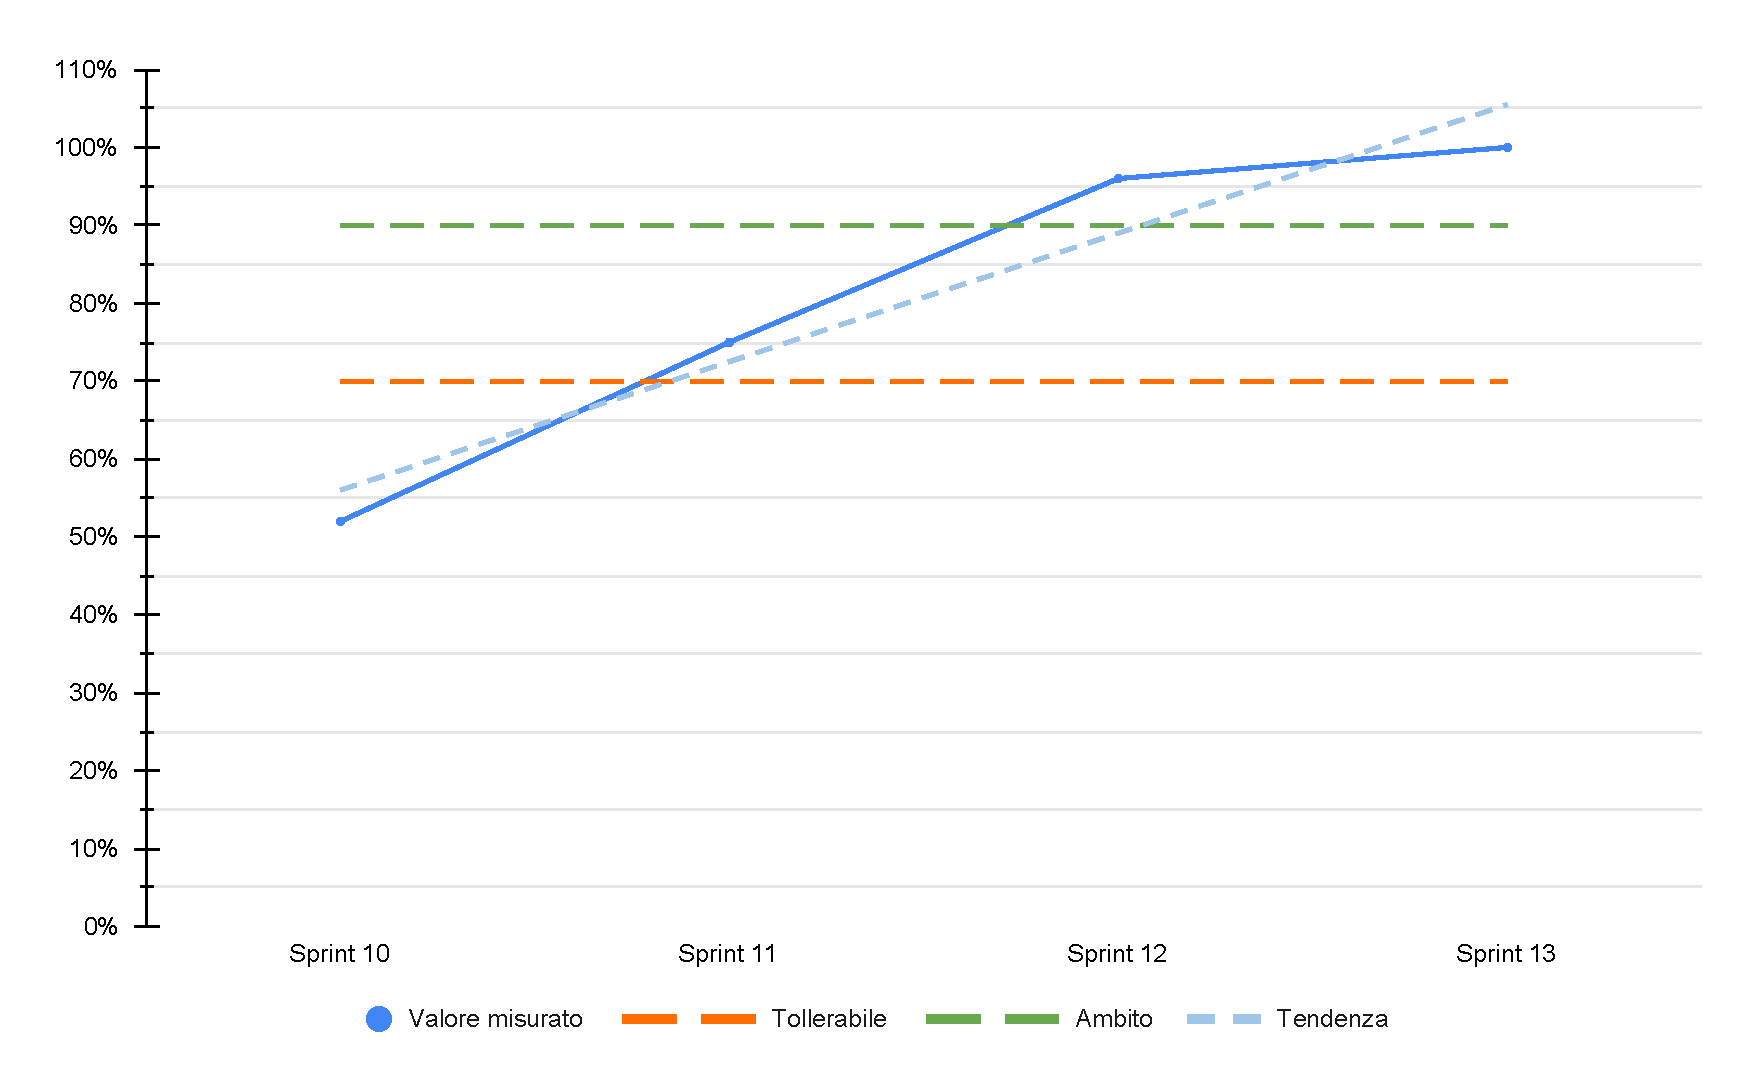
\includegraphics[width=\textwidth]{assets/adeguatezza_funzioni.pdf}
  \caption{M.PD.12 - Adeguatezza delle funzioni sviluppate}
\end{figure}

\par L'adeguatezza di una funzione si basa su tre fattori principali: conformità ai requisiti, copertura del codice e superamento dei test. Nel primo sprint della \glossario{PB} il valore misurato ha superato il 50\%, in quanto il codice \glossario{front-end} aveva già raggiunto un livello di adeguatezza tale da soddisfare gli standard previsti. A partire dallo \glossario{sprint} 11, la percentuale è cresciuta progressivamente, fino a superare la soglia desiderata nel dodicesimo sprint. Durante lo sviluppo, il team ha verificato che per ciascuna funzione:
\begin{itemize}
  \item La copertura dei test fosse superiore al 90\%;
  \item La percentuale di superamento dei test raggiungesse il 100\%;
  \item Il codice fosse conforme ai requisiti e opportunamente commentato.
\end{itemize}

\vspace{0.5\baselineskip}
\par Grazie a questi controlli, il team ha assicurato che le funzioni sviluppate fossero in linea con le aspettative.